\part{Integrali}

\chapter{Introduzione agli integrali}
Gli integrali nascono per rispondere alla seguente domanda.
\textit{Se abbiamo un grafico, come possiamo calcolare l'area di una regione di piano?}

\begin{center}
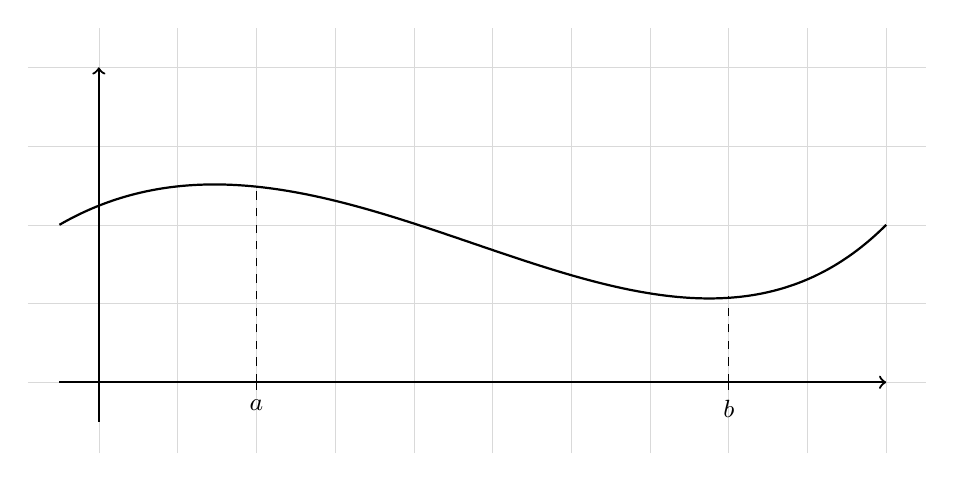
\begin{tikzpicture}
    % Coordinate
    \draw[very thin, gray!30, step=1 cm](-.9,-.9) grid (10.5,4.5);
    \coordinate (P1) at (-0.5,2);
    \coordinate (P2) at (10,2);
    % Linee
    \path [thick, black,out=30,in=225] (P1) edge (P2); % curved line
    \draw [->,thick] (-0.5,0) -- (10,0); % asse x
    \draw [->,thick] (0,-0.5) -- (0,4); % asse y
    \draw [dashed] (2,0) -- (2,2.5);
    \draw [dashed] (8,0) -- (8,1.1);
    % Writing space
    \draw (2,0) -- (2,-0.1) node [below] {\small{$a$}};
    \draw (8,0) -- (8,-0.1) node [below] {\small{$b$}};
\end{tikzpicture}
\end{center}

Se vogliamo calcolare l'area di un sotto-grafico di una funzione $f[a,b]\to\mathbb{R}$, $f(x)\geq0$ possiamo provare a confrontare la regione di piano con le aree di figure che conosciamo.
\begin{itemize}
    \item Area di un rettangolo: $A=b*h$.
    \item Area di un'unione disgiunta di rettangoli: è la somma delle aree dei singoli rettangoli.
\end{itemize}

\subsubsection{Stima dall'alto}
Se $f[a,b]\to\mathbb{R}$ è positiva e limitata allora $\exists M>0$ tale che $0\leq f(x)\leq M$, $\forall x\in[a,b]$, intuitivamente notiamo che l'area sarà maggiore di 0 e minore del rettangolo in cui è contenuta.

\begin{center}
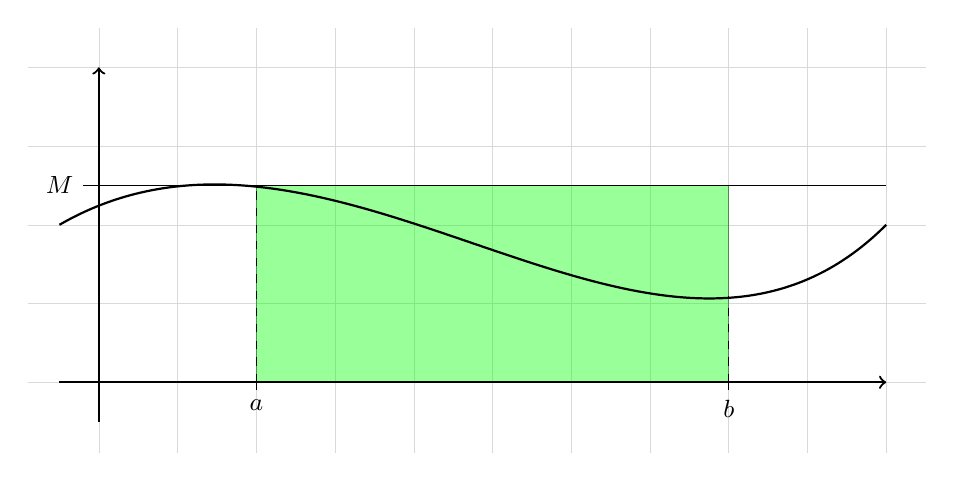
\begin{tikzpicture}
    % Decoration
    \draw[very thin, gray!30, step=1 cm](-.9,-.9) grid (10.5,4.5);
    \draw [fill=green, very thin, opacity=0.4] (2,0) rectangle (8,2.5);
    % Coordinate
    \coordinate (P1) at (-0.5,2);
    \coordinate (P2) at (10,2);
    % Linee
    \path [thick, black,out=30,in=225] (P1) edge (P2); % curved line
    \draw [->,thick] (-0.5,0) -- (10,0); % asse x
    \draw [->,thick] (0,-0.5) -- (0,4); % asse y
    \draw [dashed] (2,0) -- (2,2.5);
    \draw [dashed] (8,0) -- (8,1.1);
    \draw [-] (0,2.5) -- (10,2.5);
    % Writing space
    \draw (2,0) -- (2,-0.1) node [below] {\small{$a$}};
    \draw (8,0) -- (8,-0.1) node [below] {\small{$b$}};
    \draw (0,2.5) -- (-0.2,2.5) node [left] {\small{$M$}};
\end{tikzpicture}
\end{center}

Possiamo fare questo confronto con qualsiasi rettangolo di base $b-a$ e di altezza $M>0$ tale che $M\geq f(x)$, $\forall x\in[a,b]$.

Ovviamente, però, la stima sarà tanto migliore quanto approssimata a valori molto vicini di $f(x)$. Ovvero quando $M$ coincide con il massimo della funzione.
\begin{equation*}
    0\leq A\leq (b-a)M\hspace{1cm}M=\max_{[a,b]}f(x)
\end{equation*}

\subsubsection{Stima dal basso}
Anche in questo caso ricerchiamo la migliore stima dal basso, quindi quando $m$ coincide con il minimo della funzione.

\begin{center}
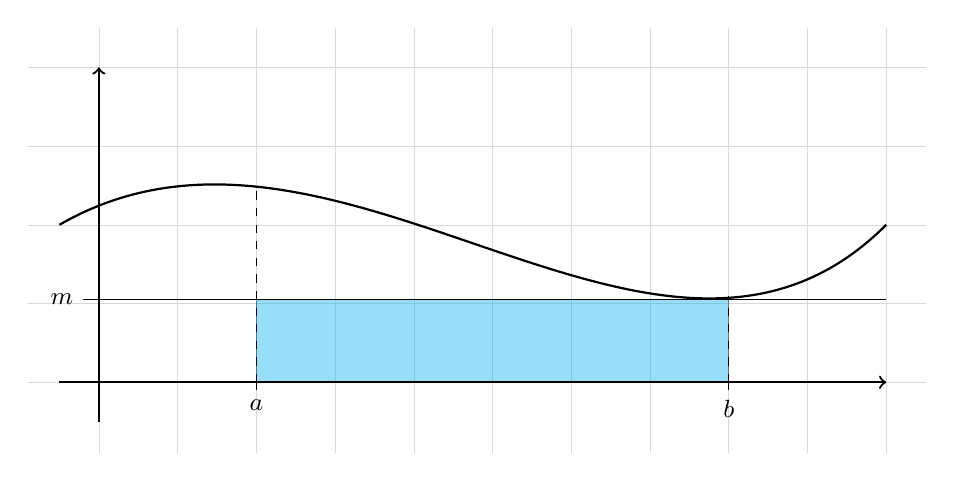
\begin{tikzpicture}
    % Decoration
    \draw[very thin, gray!30, step=1 cm](-.9,-.9) grid (10.5,4.5);
    \draw [fill=cyan, very thin, opacity=0.4] (2,0) rectangle (8,1.05);
    % Coordinate
    \coordinate (P1) at (-0.5,2);
    \coordinate (P2) at (10,2);
    % Linee
    \path [thick, black,out=30,in=225] (P1) edge (P2); % curved line
    \draw [->,thick] (-0.5,0) -- (10,0); % asse x
    \draw [->,thick] (0,-0.5) -- (0,4); % asse y
    \draw [dashed] (2,0) -- (2,2.5);
    \draw [dashed] (8,0) -- (8,1.1);
    \draw [-] (0,1.05) -- (10,1.05);
    % Writing space
    \draw (2,0) -- (2,-0.1) node [below] {\small{$a$}};
    \draw (8,0) -- (8,-0.1) node [below] {\small{$b$}};
    \draw (0,1.05) -- (-0.2,1.05) node [left] {\small{$m$}};
\end{tikzpicture}
\end{center}

\begin{equation*}
    (b-a)m\leq A\leq (b-a)M\hspace{1cm}m=\min_{[a,b]}f(x)
\end{equation*}


\subsubsection{Possiamo fare di meglio!}
Fino ad ora abbiamo usato il confronto con l'area del rettangolo migliore. \textit{Perchè non provare con la somma dell'area disgiunta di rettangoli?}

\begin{center}
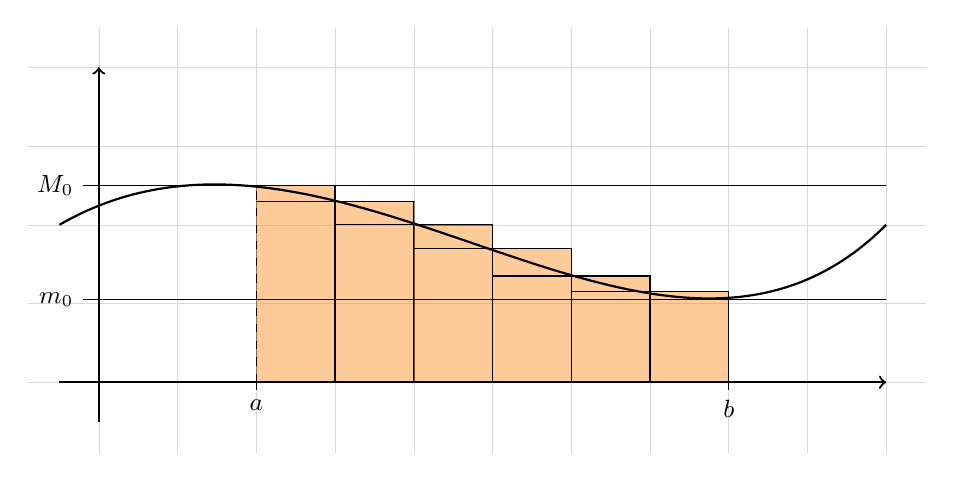
\begin{tikzpicture}
    % Decoration
    \draw[very thin, gray!30, step=1 cm](-.9,-.9) grid (10.5,4.5);
    \draw [fill=orange, very thin, opacity=0.4] (2,2.5) rectangle (3,0);
    \draw [fill=orange, very thin, opacity=0.4] (3,2.3) rectangle (4,0);
    \draw [fill=orange, very thin, opacity=0.4] (4,2) rectangle (5,0);
    \draw [fill=orange, very thin, opacity=0.4] (5,1.7) rectangle (6,0);
    \draw [fill=orange, very thin, opacity=0.4] (6,1.35) rectangle (7,0);
    \draw [fill=orange, very thin, opacity=0.4] (7,1.15) rectangle (8,0);
    % Coordinate
    \coordinate (P1) at (-0.5,2);
    \coordinate (P2) at (10,2);
    % Linee
    \path [thick, black,out=30,in=225] (P1) edge (P2); % curved line
    \draw [->,thick] (-0.5,0) -- (10,0); % asse x
    \draw [->,thick] (0,-0.5) -- (0,4); % asse y
    \draw [dashed] (2,0) -- (2,2.5);
    \draw [dashed] (8,0) -- (8,1.1);
    \draw [-] (0,1.05) -- (10,1.05);
    \draw [-] (0,2.5) -- (10,2.5);
    % Rectangle [start, end] = [(2,2.5), (8,1.1)]
    \draw [-] (2,2.5) -- (3,2.5);\draw [-] (3,0) -- (3,2.5);
    \draw[](3,2.3) rectangle (4,0);
    \draw[](4,2) rectangle (5,0);
    \draw[](5,1.7) rectangle (6,0);
    \draw[](6,1.35) rectangle (7,0);
    \draw[](7,1.15) rectangle (8,0);
    
    \draw [-] (2,2.3) -- (3,2.3);
    \draw [-] (3,2) -- (4,2);
    \draw [-] (4,1.7) -- (5,1.7);
    \draw [-] (5,1.35) -- (6,1.35);
    \draw [-] (6,1.15) -- (7,1.15);
    % Writing space
    \draw (2,0) -- (2,-0.1) node [below] {\small{$a$}};
    \draw (8,0) -- (8,-0.1) node [below] {\small{$b$}};
    \draw (0,1.05) -- (-0.2,1.05) node [left] {\small{$m_0$}};
    \draw (0,2.5) -- (-0.2,2.5) node [left] {\small{$M_0$}};
\end{tikzpicture}
\end{center}

Prendendo i minimi $m_j$ e i massimi $M_j$, produciamo la somma dei rettangoli inferiori $A_j$ e la somma dei rettangoli superiori $B_j$. Otteniamo così:
\begin{equation*}
    \sum^n_{i=1}A_i\leq A\leq \sum^n_{i=1}B_i
\end{equation*}
Ricordando di:
\begin{enumerate}
    \item Fissare $n\in\mathbb{N}$;
    \item Dividere l'intervallo $[a,b]$ in $2^n$ parti uguali.
\end{enumerate}
\begin{equation*}
    x_k=a+k\frac{b-a}{2^n}\hspace{1cm}k=0,1,...,2^n
\end{equation*}
Chiamiamo:
\begin{equation*}
    \alpha_k=\min_{[x_k,x_{k+1}]}f(x)\hspace{1cm}\beta_k=\max_{[x_k,x_{k+1}]}f(x)
\end{equation*}
Otteniamo:
\begin{equation*}
    \underline{S_n}=\sum^{2^n-1}_{k=0}\alpha_k(\frac{b-a}{2^n})\leq A \leq \overline{S_n}=\sum^{2^n-1}_{k=0}\beta_k(\frac{b-a}{2^n})
\end{equation*}
Con $\underline{S_n}$ che rappresenta le somme integrali per difetto di una partizione $\{x_0, x_n\}$ di $[a,b]$ e $\overline{S_n}$ che rappresenta le somme integrali per eccesso di una partizione $\{x_0, x_n\}$ di $[a,b]$ e $\overline{S_n}$.

All'aumentare di $n$, otteniamo un numero maggiore di intervalli e un'ampiezza inferiore degli stessi. In questo modo, restringendo il range degli intervalli, aumenta il minimo o al più resta uguale a $\alpha_k$, e al contrario, diminuisce il massimo o al più resta uguale a $\beta_k$.
Quindi $\underline{S_n}$ è crescente e $\overline{S_n}$ è decrescente, con $\underline{S_n}\leq A\leq \overline{S_n}$.
Infine per $f(x)\geq0$, $\underline{S_n}\to\underline{S}$ e $\overline{S_n}\to\overline{S}$, con $\underline{S_n}\leq A\leq \overline{S_n}$.

\begin{definition*}[Integrale]
    Sia $f[a,b]\to\mathbb{R}$ positiva e limitata, $f$ si dice integrabile (secondo Riemann) se:
    \begin{equation*}
        \exists\lim_{n\to+\infty}\frac{b-a}{2^n}\sum^{2^n-1}_{k=0}\min_{[x_k, x_{k+1}]}f(x)=\underline{S}=\overline{S}=\exists\lim_{n\to+\infty}\frac{b-a}{2^n}\sum^{2^n-1}_{k=0}\max_{[x_k, x_{k+1}]}f(x)
    \end{equation*}
    \begin{equation*}
        \underline{S}=\overline{S}=\int_a^bf(x)dx
    \end{equation*}
\end{definition*}

\begin{example}
    \begin{itemize}
        \item $f(x)=2$ su $[0,1]$
        
        Si nota sin da subito che se $f(x)$ è costante otteniamo un'area rettangolare.
        \begin{equation*}
            \int_0^12dx=1*2=2
        \end{equation*}
        Vediamo come fare applicando le definizioni:
        \begin{enumerate}
            \item Fisso $n\in\mathbb{N}$;
            \item Partiziono: \begin{equation*}x_k=a+k\frac{b-a}{2^n}=0+k\frac{1-0}{2^n}=\frac{k}{2^n}\hspace{1cm}k=0,...,2^n;\end{equation*}
            \item \begin{equation*}\alpha_k=\min_{[x_k,x_{k+1}]}f(x)=2\hspace{1cm}\underline{S_n}=\frac{1-0}{2^n}\sum^{2^n-1}_{k=0}2=\frac{1}{2^n}2\sum^{2^n-1}_{k=0}1=\frac{2^n}{2^n}2\end{equation*}
            \begin{equation*}\beta_k=\max_{[x_k,x_{k+1}]}f(x)=2\hspace{1cm}\overline{S_n}=\frac{1-0}{2^n}\sum^{2^n-1}_{k=0}2=\frac{1}{2^n}2\sum^{2^n-1}_{k=0}1=\frac{2^n}{2^n}2\end{equation*}
        \end{enumerate}
        
        \item $f(x)=x^2$ su $[0,1]$
        
        $x_k=a+k\frac{b-a}{2^n}$
        \begin{equation*}
            \alpha_k=\min_{[x_k,x_{k+1}]}f(x)=(x_k)^2=\frac{1}{2^n}\sum^{2^n-1}_{k=0}\frac{k^2}{(2^n)^2}=\frac{1}{2^{3n}}\sum^{2^n-1}_{k=0}k^2=
        \end{equation*}
        \begin{equation*}
            =\frac{1}{6}m(m+1)(2m+1)=\frac{1}{6}2^n-1(2^n)(4^n-1)
        \end{equation*}
        
        \item $f(x)=e^x$ su $[0,1]$
        
        $e^x$ è crescente e $a_k=f(x_k)=e^{x_k}$.\\
        \begin{equation*}
            \underline{S_n}=\frac{1}{2^n}\sum^{2^n-1}_{k=0}e^{x_k}=\frac{1}{2^n}\sum^{2^n-1}_{k=0}e^{\frac{k}{2^n}}=\frac{1}{2^n}\sum^{2^n-1}_{k=0}(e^{\frac{1}{2^n}})^k=\frac{1-r^{n+1}}{1-r}=\frac{1}{2^n}\frac{1-(e^{\frac{1}{2^n}})^{2n-2}}{1-e^{\frac{1}{2^n}}}=e-1    
        \end{equation*}
        \begin{equation*}
            \int^1_0e^xdx=e-1
        \end{equation*}
    \end{itemize}
\end{example}

\begin{osservation*}
    $\int_a^bf(x)dx$ è una notazione per indicare che sto integrando nella variabile $x$. Infatti:
    \begin{equation*}\int_a^bf(x)dx=\int_a^bf(t)dt=\int_a^bf(y)dy\end{equation*}
\end{osservation*}

\subsection*{Quali funzioni sono integrabili?}
Non tutte le funzioni sono integrabili. Ad esempio la \textit{funzione di Dirichlet}:
$$\begin{cases}
    1\hspace{0.5cm}se\hspace{0.5cm}x\in\mathbb{Q}\\
    0\hspace{0.5cm}se\hspace{0.5cm}x\notin\mathbb{Q}
\end{cases}\hspace{1cm}\min_{[x_k,x_{k+1}]}D(x)=0\hspace{1cm}\max_{[x_k,x_{k+1}]}D(x)=1$$

Essendo $\underline{S_n}=0$, $\overline{S_n}=1$ e $\underline{S_n}\neq \overline{S_n}$ la funzione non è integrabile.

In generale sono esempi di funzioni integrabili quelle funzioni:
\begin{enumerate}
    \item $f[a,b]\to\mathbb{R}$ monotone;
    \item $f[a,b]\to\mathbb{R}$ continue.
\end{enumerate}


\chapter{Proprietà delle funzioni integrabili}
\subsection*{Linearità dell'integrale}

$f,g$ integrabili su $[a,b]\Rightarrow\alpha f+\beta g$ è integrabile su $[a,b]$, $\forall\alpha,\beta\in\mathbb{R}$ e
\begin{equation*}
    \int^b_a[\alpha f(x)+\beta g(x)]dx=\alpha\int^b_af(x)dx+\beta\int^b_ag(x)dx
\end{equation*}

\subsection*{Additività dell'intervallo}
$[a,b]=[a,c]\cup[c,b]$

Se $f$ è integrabile su $[a,c]$ e $f$ è integrabile su $[c,b]$ allora $f$ è integrabile su $[a,b]$ e
\begin{equation*}
    \int^b_af(x)dx=\int^c_af(x)dx+\int^b_cf(x)dx
\end{equation*}

\begin{center}
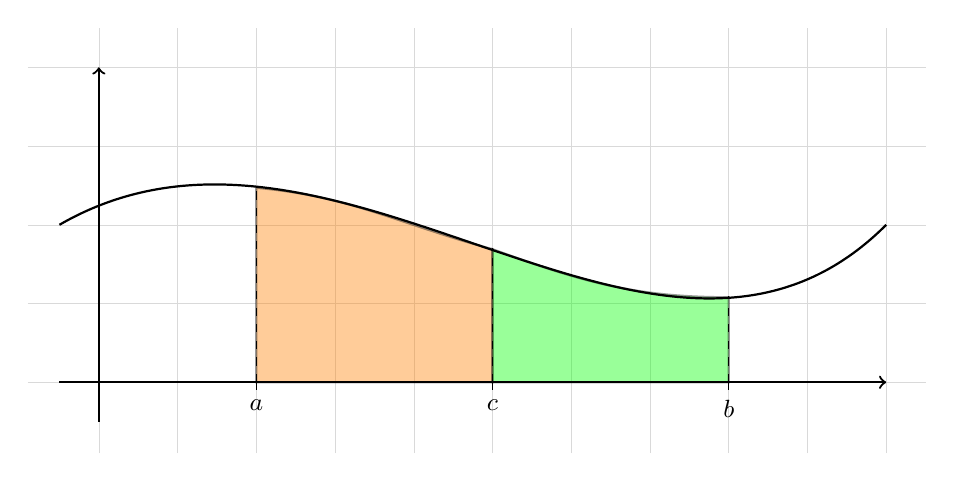
\begin{tikzpicture}
    % Decoration
    \draw[very thin, gray!30, step=1 cm](-.9,-.9) grid (10.5,4.5);
    % Decoration curve line
    \draw[thick,fill=orange, opacity=0.4] (5,0) -- (5,0) -- (2,0) -- (2,2.47) to [out=-5,in=165]  (5, 1.69) --cycle ;
    \draw[thick,fill=green, opacity=0.4] (8,0) -- (8,0) -- (5,0) -- (5,1.69) to [out=-20,in=180]  (8, 1.08) --cycle ;
    % Coordinate
    \coordinate (P1) at (-0.5,2);
    \coordinate (P2) at (10,2);
    % Linee
    \path [thick,black,out=30,in=225] (P1) edge (P2); % curved line
    \draw [->,thick] (-0.5,0) -- (10,0); % asse x
    \draw [->,thick] (0,-0.5) -- (0,4); % asse y
    \draw [dashed] (2,0) -- (2,2.5);
    \draw [dashed] (5,0) -- (5,1.7);
    \draw [dashed] (8,0) -- (8,1.1);
    % Writing space
    \draw (2,0) -- (2,-0.1) node [below] {\small{$a$}};
    \draw (5,0) -- (5,-0.1) node [below] {\small{$c$}};
    \draw (8,0) -- (8,-0.1) node [below] {\small{$b$}};
\end{tikzpicture}
\end{center}


\subsection*{Funzioni integrabili}
Se:
\begin{enumerate}
    \item $f$ è monotona;
    \item $f$ è continua;
    \item $f$ ha un numero finito di cambi di monotonia;
    \item $f$ ha un numero finito di punti di discontinuità.
\end{enumerate}
allora $f$ è integrabile.

\subsection*{Funzioni che cambiano di segno}
Se $f(x)$ cambia segno dobbiamo calcolare la somma delle aree con segno:

\begin{center}
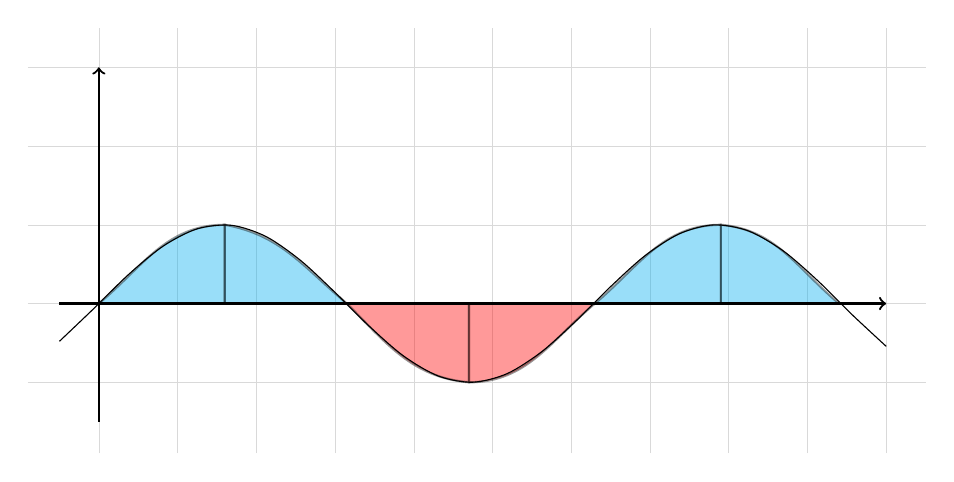
\begin{tikzpicture}
    % Decoration
    \draw[very thin, gray!30, step=1 cm](-.9,-1.9) grid (10.5,3.5);
    % Decoration curve line
    \draw[thick,fill=cyan, opacity=0.4] (1.6,0) -- (0,0) to [out=40,in=180]  (1.6, 1) --cycle ;
    \draw[thick,fill=cyan, opacity=0.4] (1.6,0) -- (3.15,0) to [out=140,in=-10]  (1.6, 1) --cycle ;
    \draw[thick,fill=cyan, opacity=0.4] (7.9,0) -- (6.3,0) to [out=40,in=180]  (7.9, 1) --cycle ;
    \draw[thick,fill=cyan, opacity=0.4] (7.9,0) -- (9.4,0) to [out=140,in=-5]  (7.9, 1) --cycle ;
    
    \draw[thick,fill=red, opacity=0.4] (4.7,0) -- (3.15,0) to [out=-45,in=-185]  (4.7, -1) --cycle ;
    \draw[thick,fill=red, opacity=0.4] (4.7,0) -- (6.3,0) to [out=-140,in=0]  (4.7, -1) --cycle ;
    % Linee
    \draw[scale=1, domain=-.5:10, smooth, variable=\x, black] plot ({\x}, {sin(deg(\x))}); % Curved line
    \draw [->,thick] (-0.5,0) -- (10,0); % asse x
    \draw [->,thick] (0,-1.5) -- (0,3); % asse y
\end{tikzpicture}
\end{center}

\begin{equation*}
    \int^b_af(x)dx=\text{ somma delle aree con segno}
\end{equation*}
\begin{itemize}
    \item se $f(x)<0$ in $[c,d]\subset[a,b]$ sottraggo l'area di questo intervallo;
    \item se $f(x)>0$ in $[c,d]\subset[a,b]$ sommo l'area di questo intervallo;
\end{itemize}

\subsection*{Monotonia}
Se $f(x)\leq g(x)$, $\forall x\in[a,b]$
\begin{enumerate}
    \item \begin{equation*}\int^b_af(x)dx\leq\int^b_ag(x)dx\end{equation*}
    \item \begin{equation*}|\int^b_af(x)dx|\leq\int^b_a|f(x)|dx\end{equation*}
    \item Per qualsiasi $f(x)$ integrabile:\begin{equation*}\int^a_af(x)dx=0\end{equation*}
    \item Per $a<b$:\begin{equation*}\int^b_af(x)dx:=-\int^a_bf(x)dx\end{equation*}
\end{enumerate}

\begin{osservation*}
\begin{equation*}
    \int^b_cf(x)dx=-\int^c_af(x)dx+\int^b_af(x)dx
\end{equation*}
\begin{center}
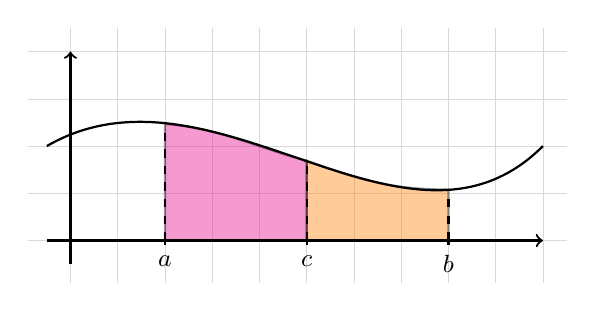
\begin{tikzpicture}[thick, scale=0.6]
    % Decoration
    \draw[very thin, gray!30, step=1 cm](-.9,-.9) grid (10.5,4.5);
    % Decoration curve line
    \draw[thick,fill=magenta, opacity=0.4] (5,0) -- (5,0) -- (2,0) -- (2,2.47) to [out=-5,in=165]  (5, 1.69) --cycle ;
    \draw[thick,fill=orange, opacity=0.4] (8,0) -- (8,0) -- (5,0) -- (5,1.69) to [out=-20,in=180]  (8, 1.08) --cycle ;
    % Coordinate
    \coordinate (P1) at (-0.5,2);
    \coordinate (P2) at (10,2);
    % Linee
    \path [thick,black,out=30,in=225] (P1) edge (P2); % curved line
    \draw [->,thick] (-0.5,0) -- (10,0); % asse x
    \draw [->,thick] (0,-0.5) -- (0,4); % asse y
    \draw [dashed] (2,0) -- (2,2.5);
    \draw [dashed] (5,0) -- (5,1.7);
    \draw [dashed] (8,0) -- (8,1.1);
    % Writing space
    \draw (2,0) -- (2,-0.1) node [below] {\small{$a$}};
    \draw (5,0) -- (5,-0.1) node [below] {\small{$c$}};
    \draw (8,0) -- (8,-0.1) node [below] {\small{$b$}};
\end{tikzpicture}
\end{center}
\end{osservation*}


\section{Teorema fondamentale del calcolo integrale 1}\label{sec:TFCI}
Sia $f[a,b]\to\mathbb{R}$ continua, poniamo $F(t)=\int^t_af(x)dx$ allora la funzione $F(t)$ è derivabile e $F'(t)=f(t)$, $\forall t\in[a,b]$.

\begin{example}\phantom{}
    \begin{itemize}
        \item $f(x)=x$ su $[0,2]$
    
        $F(t)=\int^t_0xdx=\frac{t^2}{2}$, $\forall t\in[0,2]$
        \item $f(x)=x$ su $[1,2]$
        
        $F(t)=\int^b_af(x)dx=\int^t_1xdx=\frac{t^2}{2}-\frac{1}{2}$
    \end{itemize}
\end{example}

In generale:
\begin{center}
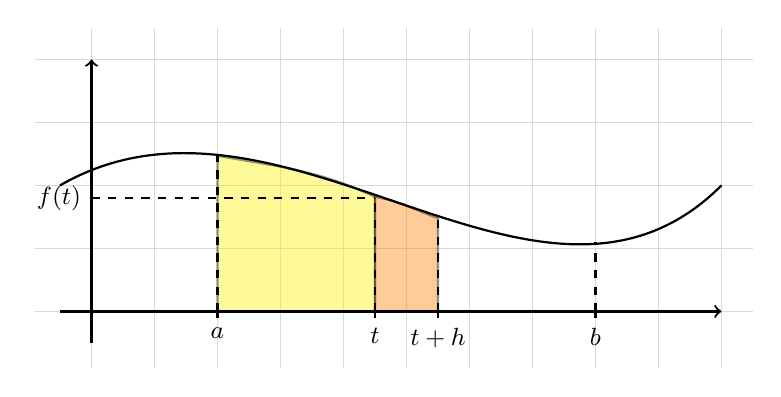
\begin{tikzpicture}[thick, scale=0.8]
    % Decoration
    \draw[very thin, gray!30, step=1 cm](-.9,-.9) grid (10.5,4.5);
    % Decoration curve line
    \draw[thick,fill=yellow, opacity=0.4] (4.5,0) -- (4.5,0) -- (2,0) -- (2,2.47) to [out=-10,in=155]  (4.5, 1.82) --cycle ;
    \draw[thick,fill=orange, opacity=0.4] (5.5,0) -- (5.5,0) -- (4.5,0) -- (4.5,1.82) to [out=-10,in=160]  (5.5, 1.48) --cycle ;
    % Coordinate
    \coordinate (P1) at (-0.5,2);
    \coordinate (P2) at (10,2);
    % Linee
    \path [thick,black,out=30,in=225] (P1) edge (P2); % curved line
    \draw [->,thick] (-0.5,0) -- (10,0); % asse x
    \draw [->,thick] (0,-0.5) -- (0,4); % asse y
    \draw [dashed] (2,0) -- (2,2.5);
    \draw [dashed] (4.5,0) -- (4.5,1.8);
    \draw [dashed] (5.5,0) -- (5.5,1.5);
    \draw [dashed] (8,0) -- (8,1.1);
    \draw [dashed] (0,1.8) -- (4.5,1.8);
    % Writing space
    \draw (2,0) -- (2,-0.1) node [below] {\small{$a$}};
    \draw (4.5,0) -- (4.5,-0.1) node [below] {\small{$t$}};
    \draw (5.5,0) -- (5.5,-0.1) node [below] {\small{$t+h$}};
    \draw (8,0) -- (8,-0.1) node [below] {\small{$b$}};
    \draw (0,1.8) -- (0,1.8) node [left] {\small{$f(t)$}};
\end{tikzpicture}
\end{center}

\begin{equation*}
    F(t)=\int^t_af(x)dx\hspace{1cm}F(a)=\int^a_af(x)dx=0\hspace{1cm}F(t+h)=\int^{t+h}_af(x)dx
\end{equation*}
Allora: \begin{equation*}F(t+h)-F(t)=\int^{t+h}_af(x)dx-\int^t_af(x)dx=\int^{t+h}_tf(x)dx\end{equation*}
Quindi: \begin{equation*}F'(t)=\lim_{h\to0}\frac{F(t+h)-F(t)}{h}=\frac{Area}{(t+h)-t}=altezza=f(t)\end{equation*}

\begin{example}\phantom{}
    \begin{itemize}
        \item $f(x)=x^2$ su $[0,2]$
        \begin{equation*}
            F_0(t)=\int^t_0x^2dx\hspace{0.3cm}\forall t\in[0,2]\hspace{1cm}F_1(t)=\int^t_1x^2dx\hspace{0.3cm}\forall t\in[1,2]
        \end{equation*}
        $x^2$ è continua in $[a,b]$ e, per il teorema fondamentale del calcolo integrale, è derivabile:
        \begin{equation*}
            F'(t)=t^2\hspace{1cm}F(t)=\frac{t^3}{3}
        \end{equation*}
        \begin{equation*}2\in[0,2]\hspace{0.5cm}F_0(2)=\int^2_0x^2dx=\frac{t^3}{3}|_{t=2}-\frac{t^3}{3}|_{t=0}=\frac{8}{3}\end{equation*}
        \begin{equation*}2\in[1,2]\hspace{0.5cm}F_1(2)=\int^2_1x^2dx=\frac{t^3}{3}|_{t=2}-\frac{t^3}{3}|_{t=1}=\frac{7}{3}\end{equation*}
        
        \item $f(x)=\sin x$ su $[0,\pi]$
        \begin{equation*}F(t)=\int^t_0\sin(x)dx\hspace{0.5cm}\forall x\in[0,\pi]\end{equation*}
        \begin{equation*}F(\pi)=\int^\pi_0\sin(x)dx\hspace{1cm}F'(t)=\sin(t)\hspace{0.5cm}\forall t\in[0,\pi]\end{equation*}
    \end{itemize}
\end{example}

\section{Primitiva}
\begin{definition*}[Primitiva]
    $F$ si dice primitiva di $f(x)$ se $F'(x)=f(x)$.
    
    Se $F(x)$ è primitiva di $f(x)$, anche $F(x)+c$ è primitiva di $f(x)$. Perchè $(F(x)+c)'=F'(x)+c'=f(x)+0=f(x)$.
    
    Bisogna quindi aggiungere che data $f(x)$ continua$\backslash$monotona esistono infinite primitive.
\end{definition*}

\begin{example}
    $f(x)=\sin(x)$
    
    $F$ è una primitiva di $f(x)$ se $F'(x)=\sin(x)$. Ad esempio $F(x)=-\cos(x)$ è una primitiva di $\sin(x)$, ma anche $G(x)=-\cos(x)+c$ è una sua primitiva $\forall c\in\mathbb{R}$.
    
    Ma quale costante dobbiamo scegliere? Sapendo che:
    \begin{equation*}
        F(\pi)=-\cos(\pi)+c\hspace{1cm}\int^a_af(x)dx=0\hspace{1cm}F(0)=\int^0_0\sin(x)dx=0
    \end{equation*}
    \begin{equation*}
        F(0)=-\cos(0)+c=-1+c=0\hspace{1cm}c=1
    \end{equation*}
    il valore della costante deve essere $1$.
    
    Scegliamo ora $F(t)=-\cos(t)+1$ con $F(\pi)=-\cos(\pi)+1=1+1=2$.
\end{example}

\subsubsection*{Come risolvo $\int^b_af(x)dx$?}

In generale data $f(x)$ trovo almeno una primitiva $G(t)$ tale che $G'(t)=g(t)$. Poi dato che $F(t)=\int^t_af(x)dx$ sappiamo $F'(t)=f(t)$. $F(t)$ è trovata come $G(t)+c$ dove $c$ è quella costante tale che $F(a)=G(a)+c=0$ ovvero $c=-G(a)$.\begin{equation*}F(t)=G(t)-G(a)\end{equation*}

\begin{definition*}
    L'\textbf{integrale definito} è tale che $\int^b_af(x)dx=G(b)-G(a)$, mentre l'\textbf{integrale indefinito} è tale che $\int^b_af(x)dx=f(x)+c$.

\end{definition*}

\section{Teorema fondamentale del calcolo integrale 2}
Se $f$ è una funzione continua su $[a,b]$ allora $\int^b_af(x)dx=G(x)]^b_a=G(b)-G(a)$ dove $G(x)$ è una qualsiasi primitiva di $f(x)$, cioè $G'(x)=f(x)$.

Se $G(x)$ è una primitiva $\int^b_af(x)dx=G(b)-G(a)$. Notiamo che otteniamo lo stesso risultato anche con la primitiva $G(x)+c$: $\int^a_bf(x)dx=G(b)+c-[G(a)+c]=G(b)-G(a)$.

\subsection*{Elenco di primitive}
\begin{table}[H]
    \centering
    \begin{tabular}{|c|c|c|}
         \hline Funzione & Derivata & Integrale\\\hline\hline
         $x^\alpha$ & $\alpha x^{\alpha-1}$ & $\frac{1}{\alpha+1}x^{\alpha +1}+c$\\\hline
         $\sin(x)$ & $\cos(x)$ & $\sin(x)+c$\\\hline
         $\cos(x)$ & $-\sin(x)$ & $-\cos(x)+c$\\\hline
         $\tan(x)$ & $\frac{1}{\cos^2(x)}$ & $\tan(x)+c$\\\hline
         $\arctan(x)$ & $\frac{1}{1+x^2}$ & $\arctan(x)+c$\\\hline
         $e^x$ & $e^x$ & $e^x+c$\\\hline
         $A^x$ & $A^x\ln(A)$ & $\frac{A^x}{\ln(A)}$\\\hline
         $\ln(|x|)$ & $\frac{1}{x}$ & $\ln(|x|)$\\\hline
    \end{tabular}
    \caption{Primitive fondamentali}
    \label{tab:primitiveFondamentali}
\end{table}

\begin{example}\phantom{}
\begin{itemize}
    \item $\int^6_2 e^xdx$\begin{equation*}e^x]^6_2=e^6-e^2\end{equation*}
    \item $\int^1_0\frac{dx}{1+x^2}$\begin{equation*}\arctan(x)]^1_0=\arctan(1)-\arctan(0)=\frac{\pi}{4}\end{equation*}
    \item $\int^{-2}_{-3}\frac{dx}{x}$\begin{equation*}\ln(|x|)]^{-2}_{-3}=\ln|-2|-\ln(-3)=\ln(2)-\ln(3)\end{equation*}
    \item $\int^2_0\frac{dx}{x^2}$\begin{equation*}\arctan(x)]^2_0=\arctan(2)-\arctan(0)\end{equation*}
    \item $\int^4_1 3x^2+6x+5 dx$\begin{equation*}3\int^4_1x^2dx+6\int^4_1xdx+5\int^4_11dx=3(\frac{x^3}{3}]^4_1)+6(\frac{x^2}{2}]^4_1)+5(x]^4_1)=\end{equation*}\begin{equation*}
        =4^3-1^3+3(4^2-1^2)+5(4-1)=123\end{equation*}
\end{itemize}
\end{example}



\section{Integrali di funzioni pari/dispari}
Gli integrali di funzioni pari e dispari vengono studiati su su intervalli simmetrici. Gli unici intervalli simmetrici rispetto all'origine si presentano nella forma $[-a,a]$ oppure $(-a,a)$ con $a>0$.

In generale:
\begin{itemize}
    \item se $f(x)$ è una funzione dispari allora l'integrale nell'intervallo simmetrico $[-a,a]$ è uguale a zero;
    \item se $f(x)$ è una funzione pari allora l'integrale nell'intervallo simmetrico $[-a,a]$ è uguale a due volte l'integrale di $f(x)$ in $[0,a]$.
\end{itemize}

Ricordando che una funzione è dispari se $f(-x)=-f(x)$ mentre è pari se $f(-x)=f(x)$ capiamo il perchè di tali affermazioni.

Calcoliamo $\int^a_{-a}f(x)dx$.

Si ha per l'additività dell'integrale:
\begin{equation*}\int^a_{-a}f(x)dx=\int^0_{-a}f(x)dx+\int^a_0f(x)dx\end{equation*}

Analizziamo $\int^0_{-a}f(x)dx$ e facciamo un cambio di variabile $t=-x$. Quindi $dt=-dx$ e $x=-a$ e $t=a$ per cui:
\begin{equation*}\int^0_{-a}f(x)dx=\int_a^0f(-t)(-dt)=-\int_a^0f(-t)dt=\int^a_0f(-t)dt\end{equation*}
Se la funzione è \textit{dispari} si ha $f(-t)=-f(t)$ per cui:
\begin{equation*}
    \int^0_{-a}f(x)dx=\int^a_0(-f(t))dt=-\int^a_0f(t)dt
\end{equation*}

e quindi:
\begin{equation*}
    \int^a_{-a}f(x)dx=-\int^a_0f(x)dx+\int^a_0f(x)dx=0
\end{equation*}
Se la funzione è \textit{pari} si ha $f(-t)=f(t)$ per cui:
\begin{equation*}
    \int^0_{-a}f(x)dx=\int^a_0f(t)dt
\end{equation*}

e quindi:
\begin{equation*}
    \int^a_{-a}f(x)dx=\int^a_0f(x)dx+\int^a_0f(x)dx=2\int^a_0f(x)dx    
\end{equation*}

Possiamo quindi riassumere che:
\begin{itemize}
    \item se $f$ è pari $F(t)=\int^t_0f(x)dx$ è dispari;
    \item se $f$ è dispari $F(t)=\int^t_0f(x)dx$ è pari;
    \item se $f$ è pari $\int^a_{-a}f(x)dx=2\int^a_0f(x)dx$;
    \item se $f$ è dispari $\int^a_{-a}f(x)dx=0$;
\end{itemize}

\begin{example}
    Determinare se la seguente funzione è $>, <$ o $=$ a zero. $\int^3_{-3}[x^2\sin(x)+3|x^6|]dx$
    
    $x^2\sin(x)$ è dispari mentre $|x^6|$ è pari quindi:
    \begin{equation*}
        \int^3_{-3}x^2\sin(x)+\int^3_{-3}3|x^6| = 6\int^3_{-3}|x^6|dx = 6\int^3_0x^6dx > 0
    \end{equation*}
\end{example}




\chapter{Metodi risolutivi}
Prima di presentare i metodi per risolvere un'integrale, mostriamo qualche soluzione delle seguenti forme generali degli integrali:
\begin{table}[H]
    \centering
    \begin{tabular}{|c|c|}
         \hline Integrale & Soluzione\\\hline\hline
         $\int\frac{dx}{ax+b}$ & $\frac{1}{a}\ln(ax+b)$\\\hline
         $\int\frac{f'(x)}{f(x)}dx$ & $\ln(f(x))$\\\hline
         $\int e^{ax}dx$ & $\frac{1}{a}e^{ax}$\\\hline
         $\int g'(x)\sin(g(x))dx$ & $-\cos(g(x))$\\\hline
         $\int f'(x)\cos(f(x))dx$ & $\sin(f(x))$\\\hline
         $\int \frac{1}{\alpha^2(x-x_0)^2+\beta^2} dx$ & $\frac{1}{\alpha\beta}\arctan(\frac{\alpha}{\beta}(x-x_0))$\\\hline
    \end{tabular}
    \caption{Integrali da ricordare}
    \label{tab:integraliDaRicordare}
\end{table}
\section{Cambio di variabile}
In generale per impostare un cambio di variabile di un'integrale scriviamo:
\begin{align*}
    y=g(x)\\dy=g'(x)dx
\end{align*}

In presenza dell'integrale definito vogliamo ottenere un valore numerico dell'area e quindi calcolare il valore della primitiva nell'intervallo $[a,b]$; più nello specifico $F(y)]^b_a=F(b)-F(a)$. 

Con l'integrale indefinito, invece, dobbiamo ottenere una funzione nella variabile $x$; quindi una volta calcolata la primitiva con la sostituzione, dobbiamo riportare la x al valore originale. Ovvero se applichiamo la sostituizione con $y=x^3$ dopo aver calcolato la primitiva sostituiamo nella funzione $y$ con $x^3$.

\begin{example}\phantom{}
\begin{itemize}
    \item $\int^4_1e^{3x}dx$\begin{equation*}y=3x\hspace{0.5cm}dy=3dx\hspace{0.5cm}dx=\frac{1}{3}dy\end{equation*}
    \begin{equation*}\int^{3*4}_{3*1}e^y\frac{1}{3}dy=\frac{1}{3}\int^{12}_3e^ydy=\frac{1}{3}(e^12-e^3)\end{equation*}
\end{itemize}
\end{example}

\section{Integrazione per parti}
Siano $f$ e $g[a,b]\to\mathbb{R}$ continue, una prima idea è quella di svolgere la derivata di un prodotto: $(f(x)g(x))'=f'(x)g(x)+f(x)g'(x)$. Ottengo in questo modo $\int (f(x)g(x))'dx=\int f'(x)g(x)dx+\int f(x)g'(x)dx$. E con l'integrale definito ottengo $\int^b_a (f(x)g(x))'dx=\int^b_a f'(x)g(x)dx+\int^b_a f(x)g'(x)dx=f(b)g(b)-f(a)g(a)$. Quindi:
\begin{equation*}
    \int^b_a f'(x)g(x)dx=f(b)g(b)-f(a)g(a)-\int^b_a f(x)g'(x)dx
\end{equation*}
che può anche essere scritto come:
\begin{equation*}
    \int^b_a f'g=fg]^b_a-\int^b_a fg'\hspace{1cm}\text{oppure}\hspace{1cm}\int f'g=fg-\int fg'
\end{equation*}

\begin{osservation*}
    Quando si applica l'integrazione per parti si consiglia di scrivere la formula "semplificata" $\int f'g=fg-\int fg'$.
    
    Nel caso di integrali del tipo $P(x)(e^x/\cos(x)/\sin(x))dx$ dove $P(x)$ è un polinomio si consiglia di derivare $P(x)$ (ovvero $g(x)=P(x)$) e di integrare $e^x/\cos(x)/\sin(x)$ (ovvero $f'(x)=e^x/\cos(x)/\sin(x)$).
\end{osservation*}

\begin{example}\phantom{}
\begin{itemize}
    \item $\int xe^xdx$\\Imposto $e^x$ come l'integrale $f(x)$ e $x$ come la derivata: $g(x)$\begin{equation*}f'(x)=e^x\hspace{.5cm}g(x)=x\hspace{.5cm}\Longrightarrow\hspace{.5cm}f(x)=e^x\hspace{.5cm}g'(x)=1\end{equation*}Applico la formula dell'integrazione per parti ($\int f'g=fg-\int fg'$):\begin{equation*}xe^x-\int e^xdx=xe^x-e^x+c=e^x(x-1)+c\end{equation*}
    
    \item $\int\frac{x^2}{2}e^xdx$\begin{equation*}f'(x)=e^x\hspace{.5cm}g(x)=\frac{x^2}{2}\hspace{.5cm}\Longrightarrow\hspace{.5cm}f(x)=e^x\hspace{.5cm}g'(x)=x\end{equation*}\begin{equation*}xe^x-\int e^xdx=e^x(x-1)+c\end{equation*}
    
    
\end{itemize}
\end{example}

\subsection*{Formula dell'esponenziale}
E' possibile inoltre anche applicare una formula particolare per tutti quegli integrali nella forma:
\begin{equation*}
    \int P(x)e^{Ax}=Q(x)e^{Ax}+c
\end{equation*}
Dove $Q(x)$ è un polinomio da trovare in base al grado di $P(x)$ e tale che:\begin{equation*}Q'_n(x)+AQ_n(x)=P(x)\end{equation*} 
\begin{example}
    $xe^xdx$\begin{equation*}P(x)=x\hspace{.5cm}Ax=x\hspace{.5cm}A=1\end{equation*}
    Ora dobbiamo trovare $Q_1(x)$ (dove 1 rappresenta il grado del polinomio) tale che $Q'_1(x)+AQ_1(x)=P(x)$.
    
    Essendo $P(x)$ di primo grado $Q_1(x)=bx+c$ tale che $Q'(x)+Q(x)=x$.\\Quindi $Q'_1(x)=b$ e $P(x)=bx+b+c$ ovvero $bx+b+c=x$:
    
    $\begin{cases}b=1\\b+c=0\end{cases}\begin{cases}b=1\\c=-1\end{cases}$\\
    $Q(x)=bx+c=x-1$ e come soluzione dell'integrale $\int xe^xdx=(x-1)e^x+c$.
\end{example}


\section{Integrali razionali}
Come possiamo risolvere $\int\frac{P(x)}{Q(x)}dx$ dove $P$ e $Q$ sono due polinomi?

Se $Q'(x)=P(x)$ la risolviamo tramite il logaritmo:\begin{equation*}\int\frac{Q'(x)}{Q(x)}=\ln(Q(x))+c\end{equation*}
Se ciò non avviene la soluzione dell'integrale dipenderà dal grado dei polinomi: se il grado di $P(x)$ è maggiore del grado di $Q(x)$ allora dividiamo i polinomi; invece quando il grado di $P(x)$ è minore del grado di $Q(x)$ studiamo due possibili casi:
\begin{itemize}
    \item Quando $Q$ è un polinomio di $1^o$ grado;
    \item Quando $Q$ è un polinomio di $2^o$ grado.
\end{itemize}

\subsection*{Polinomi di grado 1}
Gli integrali razionali di grado 1 sono nella forma $\int\frac{Ax+B}{Cx+D}dx$. Qui distinguiamo due casi quando $A=0$ e quando $A\neq0$:
\begin{itemize}
    \item Per $A=0$ otteniamo $\int\frac{B}{Cx+D}dx$. Ora se:
    \begin{itemize}
        \item $C=0$ : \begin{equation*}\int\frac{B}{D}dx=\frac{B}{D}x+c\end{equation*}
        \item $C\neq0$ : \begin{equation*}\int\frac{B}{Cx+D}dx=B\int\frac{1}{Cx+D}=\frac{B}{C}\ln(|Cx+D|)+c\end{equation*}
    \end{itemize}
\end{itemize}    
    \begin{example}\phantom{}
    \begin{itemize}
        \item $\int\frac{2}{3x-6}dx$\begin{equation*}\frac{2}{3}\int\frac{1}{x-2}dx=\frac{2}{3}\ln|x-2|+c\end{equation*}
        \item $\int\frac{2}{3x-5}dx$\begin{equation*}\frac{2}{3}\int\frac{1}{x-\frac{5}{3}}=\frac{2}{3}\ln|x-\frac{5}{3}|+c\end{equation*}
    \end{itemize}
    \end{example}
Se invece:
\begin{itemize}
    \item $A\neq0$ otteniamo $\int\frac{Ax+B}{Cx+D}dx$. Ora se:
    \begin{itemize}
        \item $C=0$ : \begin{equation*}\int\frac{Ax+B}{D}=\frac{1}{D}\int Ax+Bdx=\frac{1}{D}(A\frac{x^2}{2}+Bx)+c\end{equation*}
        \item $C\neq 0$ : \begin{equation*}\int\frac{Ax+B}{Cx+D}=\alpha+\frac{\beta}{Cx+D}\end{equation*}
        Infatti tramite semplici passaggi algebrici possiamo scivere:
        \begin{equation*}Ax+B=\frac{A}{C}(Cx)+B=\frac{A}{C}(Cx)+\frac{AD}{C}-\frac{AD}{C}+B\end{equation*}
        e la frazione:
        \begin{equation*}\frac{Ax+B}{Cx+D}=\frac{A}{C}\frac{Cx+D}{Cx+D}+\frac{B-\frac{AD}{C}}{Cx+D}\end{equation*}
        dove $\frac{A}{C}=\alpha$ mentre $\frac{B-\frac{AD}{C}}{Cx+D}=\beta$.
        Quindi:
        \begin{equation*}\int\frac{Ax+B}{Cx+D}dx=\int\frac{A}{C}dx+\int\frac{\frac{BC-AD}{C}}{Cx+D}dx\end{equation*}
        \begin{example}$\int\frac{3x+8}{2x-5}dx$\begin{equation*}\int\frac{3}{2}dx+\frac{8*2-3(-5)}{2}\int\frac{1}{2x-5}dx=\frac{3}{2}x+\frac{31}{4}\ln|2x+5|+c\end{equation*}
        \end{example}
    \end{itemize}
\end{itemize}
    


\subsection*{Polinomi di grado 2}
L'integrale razionale di secondo grado si presenta nella forma $\int\frac{ax+b}{Ax^2+Bx+C}$, dove se:
\begin{itemize}
    \item $A=0$ : lo risolviamo tramite gli integrali razionali di primo grado visti precedentemente;
    \item $A\neq0$ : $Q(x)=x^2+bx+c$ e scrivo $Q(x)=0$ ovvero $x^2+bx+c=0$. Con un'equazione siffatta abbiamo tre possibili opzioni:
    $$\begin{cases}\text{due radici } x_1\neq x_2\\1 \text{ radice doppia }x_1=x_2\\\text{complessi coniugati }x_1,x_2=\alpha\pm i\beta
    \end{cases}$$
    Ricordando che $x_i=\frac{-b\pm\sqrt{b^2-4ac}}{2a}$ se:
    $$\Delta = b^2-4ac\begin{cases}>0\hspace{.5cm}x_1,x_2\in\mathbb{R}\hspace{.5cm}x_1\neq x_2\\
    =0\hspace{.5cm}x_1,x_2\in\mathbb{R}\hspace{.5cm}x_1=x_2\\
    <0 x_1,x_2=\alpha\pm c\beta
    \end{cases}$$
    A questi tre casi corrispondono tre metodi risolutivi diversi.
\end{itemize}

\subsubsection{Radici reali e distinte}
Otteniamo due radici reali e distinte quando $b^2-4ac>0$.
\begin{example} $\int\frac{dx}{x^2-5x+6}$
\begin{equation*}x_1,x_2=\frac{5\pm\sqrt{25-24}}{2}=\frac{5\pm1}{2}\hspace{1cm}x^2-5x+6=(x-3)(x-2)\end{equation*}
Devo trovare A e B tali che:
\begin{equation*}\frac{1}{(x-3)(x-2)}=\frac{A}{x-3}+\frac{B}{x-2}\hspace{1cm}\frac{A(x-2)+B(x-3)}{(x-3)(x-2)}\end{equation*}
Vogliamo ottenere $1=A(x-2)+B(x-3)$. Ora se $x=2$, $B=-1$ mentre se $x=3$, $A=1$.
\begin{equation*}\int\frac{dx}{x^2-5x+6}=\int\frac{dx}{(x-3)(x-2)}=\int\frac{1}{x-3}-\frac{1}{x-2}dx=\ln|\frac{x-3}{x-2}|+c\end{equation*}
\end{example}

In generale:
\begin{equation*}\int\frac{dx}{x^2-bx+c}dx=\int\frac{dx}{(x-x_1)(x-x_2)}=\int\frac{A}{x-x_1}+\frac{B}{x-x_2}dx\end{equation*}
A e B si trovano perchè $1=A(x-x_1)+B(x-x_2)$. Se $x=x_2$, $1=B(x_2-x_1)$ mentre se $x=x_1$, $1=A(x_1-x_2)$. Con $A=\frac{1}{x_1-x_2}$ e $B=\frac{1}{x_2-x_1}$.
\begin{equation*}\int\frac{1}{x_1-x_2}\frac{1}{x-x_1}+\frac{1}{x_2-x_1}\frac{1}{x-x_2}dx=\frac{1}{x_1-x_2}\int\frac{1}{x-x_1}dx+\frac{1}{x_2-x_1}\int\frac{1}{x-x_2}dx=\end{equation*}
\begin{equation*}=\frac{1}{x_1-x_2}\int\frac{1}{x-x_1}-\frac{1}{x-x_2}dx=\frac{1}{x_1-x_2}(\ln|x-x_1|-\ln|x-x_2|)+c\end{equation*}
In definitiva:
\begin{equation*}
\int\frac{dx}{x^2+bx+c}=\frac{1}{x_1-x_2}\ln|\frac{x-x_1}{x-x_2}|+c
\end{equation*}

\subsubsection{Radici reali e coincidenti}
Otteniamo due radici reali e coincidenti quando $b^2=4ac$.
\begin{example} $\int\frac{dx}{x^2-4x+4}$
\begin{equation*}x_1,x_2=\frac{4\pm\sqrt{16-16}}{2}\hspace{1cm}2(x^2-4x+4)=(x-2)^2\end{equation*}
\begin{equation*}\int\frac{dx}{x^2-4x+4}=\int\frac{dx}{(x-2)^2}=\frac{(x-2)^{-2+1}}{-2+1}=\frac{(x-2)^{-1}}{-1}=-\frac{1}{x-2}+c\end{equation*}
\end{example}

In generale:
\begin{equation*}
    \int\frac{dx}{x^2+bx+c}=\frac{-1}{x+\frac{b}{2}}
\end{equation*}

\subsubsection{Radici complesse e convergenti}
Otteniamo due radici complesse e convergenti quando $b^2-4ac<0$. Osserviamo che:
\begin{equation*}x^2-bx+c = x^2+bx+\frac{b^2}{4}-\frac{b^2}{4}+c=(x-\frac{b}{2})^2+\frac{4c-b^2}{4}=\frac{4c-b^2}{4}[(\frac{x+\frac{b}{2}}{\frac{\sqrt{4c-b^2}}{2}})^2+1]=\end{equation*}
\begin{equation*}=\frac{4c-b^2}{4}[\frac{\frac{2x+b}{2}}{\frac{\sqrt{4c-b^2}}{2}}+1]=\frac{4c-b^2}{4}[(\frac{2x+b}{\sqrt{4c+b^2}})^2+1]=\end{equation*}
\begin{equation*}=\frac{4}{4c-b^2}-\int\frac{1}{(\frac{2x-b}{\sqrt{4c-b^2}})^2+1}dx=\frac{4}{4c-b^2}\frac{\sqrt{4c-b^2}}{2}\arctan(\frac{2x+b}{\sqrt{4c-b^2}})+c\end{equation*}
In definitiva:
\begin{equation*}
    \int\frac{dx}{x^2+bx+c}dx=\frac{2}{\sqrt{4c-b^2}}\arctan(\frac{2x+b}{\sqrt{4c-b^2}})+c
\end{equation*}


\chapter*{Esercizi svolti}
\addcontentsline{toc}{chapter}{Esercizi svolti}
\begin{exercise}[Cambio di variabile]\phantom{}
\begin{enumerate}
    \item $\int^\pi_0 \cos(6x)dx$\begin{equation*}y=6x\hspace{0.5cm}dy=6dx\hspace{0.5cm}dx=\frac{1}{6}dy\end{equation*}\begin{equation*}\int^{6\pi}_0\cos(\pi)\frac{dy}{6}=\frac{\sin(y)}{6}]^{6\pi}_0=\frac{1}{6}(\sin(6\pi)-\sin(0))\end{equation*}
    \item $\int e^{x^3}$\begin{equation*}y=x^3\hspace{.5cm}dy=3x^2dx\hspace{.5cm}dx=\frac{dy}{3x^2}\end{equation*}
    \begin{equation*}\int x^2e^y\frac{dy}{3x^2}=\frac{1}{3}\int e^ydy=\frac{1}{3}e^y+c=\frac{1}{3}e^{x^3}+c\end{equation*}
    \item $\int x^6\sin(x^7)dx$\begin{equation*}y=x^7\hspace{.5cm}dy=7x^6dx\hspace{.5cm}dx=\frac{dy}{7x^6}\end{equation*}
    \begin{equation*}\int x^6\sin(x^7)\frac{dx}{7x^6}=\int -\cos(y)\frac{dy}{7}=\frac{-\cos(x^7)}{7}+c\end{equation*}
    \item $\int\frac{dx}{ax+b}$\begin{equation*}y=ax+b\hspace{.5cm}dy=adx\hspace{.5cm}dx=\frac{dy}{a}\end{equation*}
    \begin{equation*}\int\frac{1}{y}\frac{dy}{a}=\frac{1}{a}\int\frac{dy}{y}=\frac{1}{a}\ln|y|+c=\frac{1}{a}\ln(|ax+b|)+c\end{equation*}
    \item $\int\frac{4x+6}{x^2+3x+6}dx$\begin{equation*}(x^2+3x+6)'=2x+3\hspace{.5cm}4x+6=2(2x+3)\end{equation*}
    \begin{equation*}2\int\frac{2x+3}{x^2+3x+6}dx=\hspace{.5cm} y=x^2+3x+6\hspace{.5cm}dy=(2x+3)dx\end{equation*}
    \begin{equation*}2\int\frac{dy}{y}=2\ln|y|+c=2\ln(x^2+2x+6)+c\end{equation*}
    \item $\int \ln(x)dx$
    \begin{equation*}y=\ln(x)\hspace{1cm}x=e^x\hspace{1cm}dx=e^ydy\end{equation*}
    \begin{equation*}\int\ln(e^y)e^ydy=\int ye^ydy\end{equation*}
\end{enumerate}
\end{exercise}


\begin{exercise}[Metodi risolutivi]\phantom{}
\begin{enumerate}
    \item $\int\frac{1}{4x^2-2x+1}dx$
    
    Vogliamo scrivere $4x^2-2x+1$ come $\alpha^2(x-x_0)^2+\beta^2$. Questa operazione è possibile in quanto $a>0$ e $\Delta=b^2-4ac=4-4*4=-12<0$.
    
    Scriviamo:\begin{equation*}\alpha^2(x-x_0)^2+\beta^2=\alpha^2x^2+\alpha^2x_0^2-2\alpha^2x_0x+\beta^2=\alpha^2x^2-2\alpha^2x_0x+\alpha^2x_0+\beta^2\end{equation*}\begin{equation*}4x^2-2x+1=\alpha^2x^2-2\alpha^2x_0x+\alpha^2x_0+\beta^2\end{equation*}
    $$\begin{cases}4=\alpha^2\\-2=-2\alpha^2x_0\\1=\alpha^2x_0+\beta^2\end{cases}\begin{cases}\alpha=2\\x_0=\frac{1}{4}\\\beta=\frac{\sqrt{3}}{2}\end{cases}$$
    
    Otteniamo così:
    \begin{equation*}
        \int\frac{1}{2^2(x-\frac{1}{4})^2+(\frac{\sqrt{3}}{2})^2}dx=\frac{1}{\sqrt{3}}\arctan(\frac{4}{\sqrt{3}}(x-\frac{1}{4}))
    \end{equation*}
\end{enumerate}
\end{exercise}

\begin{exercise}[Integrazione per parti]\phantom{}
    \begin{enumerate}
        \item $\int x^3e^xdx$
        \begin{equation*}f'(x)=e^x\hspace{.5cm}g(x)=x^3\hspace{.5cm}\Longrightarrow\hspace{.5cm}f(x)=e^x\hspace{.5cm}g'(x)=3x^2\end{equation*}
        \begin{equation*}\int x^3e^xdx = x^3e^x-\int 3x^2e^xdx\end{equation*}
        \item[] $\int 3x^2e^xdx$
        \begin{equation*}f'(x)=e^x\hspace{.5cm}g(x)=3x^2\hspace{.5cm}\Longrightarrow\hspace{.5cm}f(x)=e^x\hspace{.5cm}g'(x)=6x\end{equation*}
        \begin{equation*}\int 3x^2e^xdx = 3x^2e^x-\int 6xe^xdx\end{equation*}
        \item[] $\int 6xe^xdx$
        \begin{equation*}f'(x)=e^x\hspace{.5cm}g(x)=6x\hspace{.5cm}\Longrightarrow\hspace{.5cm}f(x)=e^x\hspace{.5cm}g'(x)=6\end{equation*}
        \begin{equation*}\int 6xe^xdx = 6xe^x-\int 6e^x\end{equation*}
        \\
        \begin{equation*}
            \int x^3e^xdx = x^3e^x-3x^2e^x+6xe^x+c
        \end{equation*}
        
        \item $\int x\cos(2x)dx$
        \begin{equation*}f'(x)=\cos(2x)\hspace{.5cm}g(x)=x\hspace{.5cm}\Longrightarrow\hspace{.5cm}f(x)=\frac{\sin(2x)}{2}\hspace{.5cm}g'(x)=1\end{equation*}
        \begin{equation*}\int x\cos(2x)dx = \frac{x\sin(2x)}{2}-\int\frac{\sin(2x)}{2}dx=\frac{x\sin(2x)}{2}-\frac{1}{2}\frac{-\cos(2x)}{2}+c\end{equation*}
        
        \item $\int \ln(x)dx$
        \begin{equation*}f'(x)=1\hspace{.5cm}g(x)=\ln(x)\hspace{.5cm}\Longrightarrow\hspace{.5cm}f(x)=x\hspace{.5cm}g'(x)=\frac{1}{x}\end{equation*}
        \begin{equation*}\int\ln(x)dx = x\ln(x)-\int x\frac{1}{x}dx = x\ln(x)-\int 1dx = x\ln(x)-x+c \end{equation*}
    \end{enumerate}
\end{exercise}


\begin{exercise}[Formula dell'esponenziale]\phantom{}
\begin{enumerate}
    \item $\int x^3e^xdx$
    
    Ricordiamo che $\int P(x)e^{Ax}dx=Q(x)e^{Ax}$.\\
    Dato $P_3(x)$ in $\int x^3e^xdx$ cerco $Q_3(x)$ tale che $Q'(x)+Q(x)=x^3$:
    \begin{equation*}Q(x)=ax^3+bx^2+cx+d\hspace{.5cm}\text{e}\hspace{.5cm}Q'(x)=3ax^2+2bx+c\end{equation*}
    \begin{equation*}Q'(x)+Q(x)=P(x) \implies (3ax^2+2bx+c)+ax^3+bx^2+cx+d=x^3\end{equation*}
    $$\begin{cases}ax^3=x^3\\3ax^2+bx^2=0\\2bx+cx=0\\c+d=0\end{cases}\begin{cases}a=1\\b=-3\\c=6\\d=-6\end{cases}$$
    \begin{equation*}\int x^3e^xdx=(x^3-3x^2+6x-6)e^x+c\end{equation*}
    
    \item $\int x^2e^{3x}$
    
    Dato $P_2(x)=x^2$ cerco $Q_2(x)$ tale che $Q'_2(x)+3Q_2(x)=P(x)$:
    \begin{equation*}Q_2(x)=ax^2+bx+c\hspace{1cm}Q'_2(x)=2ax+b\end{equation*}
    \begin{equation*}Q'_2(x)+3Q_2(x)=P(x) \implies 2ax+b+3ax^2+3bx+3c=x^2\end{equation*}
    $$\begin{cases}3ax^2=x^2\\2ax+3bx=0\\b+3c=0\end{cases}\begin{cases}a=\frac{1}{3}\\b=-\frac{2}{9}\\c=\frac{2}{27}\end{cases}$$
    \begin{equation*}
        \int x^2e^{3x} = (\frac{1}{3}x^2-\frac{2}{9}x+\frac{2}{27})e^{3x}+c
    \end{equation*}
\end{enumerate}
\end{exercise}

\begin{exercise}[Integrali razionali]\phantom{}
\begin{enumerate}
    \item $\int\frac{6x+8}{3x-5}dx$
    \begin{equation*}\frac{6x-8}{3x-5}=\frac{\frac{6}{3}3x+8}{3x-5}=\frac{2(3x-5)+5*2+8}{3x-5}=2+\frac{18}{3x-5}\end{equation*}
    \begin{equation*}\int 2+\frac{18}{3x-5}dx=2x+\frac{18}{3}\ln(3x-5)+c\end{equation*}
    
    \item $\int^1_0\frac{2x+6}{x-3}dx$
    \begin{equation*}\frac{2x+6}{x-3}=\frac{2(x-3)+3*2+6}{x-3}=2+12\frac{1}{x-3}\end{equation*}
    \begin{equation*}\int2+\frac{12}{x-3}dx=2x]^1_0+12\ln(x-3)]^1_0=2+12\ln(2)-12\ln(3)=2-12\ln(\frac{2}{3})\end{equation*}
\end{enumerate}
\end{exercise}

\begin{exercise}[Integrali difficili]\phantom{}
\begin{enumerate}
    \item $\int\sin/\cos ^\alpha(x)dx$
    
    Dipende dal valore dell'esponenziale. Ovvero se $\alpha$ è pari si scompone la funzione e si prosegue per parti, se $\alpha$ è dispari si scompone la funzione e si applica la sostituzione.
    
    \item $\int\cos^4(x)dx$
    \begin{equation*}\int\cos^3(x)\cos(x)dx\hspace{.5cm}\text{Per parti}\hspace{.5cm}\sin(x)\cos^3(x)+3\int\sin^2(x)\cos^2(x)dx\end{equation*}
    Non ci resta che studiare $\int\sin^2(x)\cos^2(x)dx$:
    \begin{equation*}\int(1-\cos^2(x))\cos^2(x)dx\hspace{1cm}\int\cos^2(x)-\cos^4(x)dx\end{equation*}
    Abbiamo ottenuto la funzione di partenza $\int\cos^4(x)dx$ che possiamo portare al primo membro e integrare $\int\cos^2(x)dx$:
    \begin{equation*}4\int\cos^4(x)dx=\cos^3(x)\sin(x)+3\int\cos^2(x)dx\end{equation*}
    \begin{equation*}
        \int\cos^4(x)dx=\frac{\cos^3\sin(x)}{4}+\frac{3}{8}(\sin(x)\cos(x)+x)+c
    \end{equation*}
    
    \item $\int\cos^5(x)dx$
    \begin{equation*}\int\cos^4(x)\cos(x)\hspace{1cm}\int[\cos^2(x)]^2\cos(x)dx\end{equation*}
    Ricordando che $cos^2(x)=1-\sin^2(x)$ otteniamo:
    \begin{equation*}\int(1-\sin^2(x))^2\cos(x)dx\end{equation*}
    Con la sostituzione $y=\sin(x)$, $dy=\cos(x)dx$, $dx=\frac{dy}{\cos(x)}$ otteniamo:
    \begin{equation*}\int(1-y^2)^2dy\hspace{1cm}\int y^4-2y^2+1dy\hspace{1cm}\frac{y^5}{5}-\frac{2y^3}{3}+y\end{equation*}
    Riportando in funzione di $x$:
    \begin{equation*}
        \int\cos^5(x)dx = \frac{\sin^5(x)}{5}-\frac{2}{3}\sin^3(x)+\sin(x)+c
    \end{equation*}
\end{enumerate}
\end{exercise}